% "Станет проще"

\documentclass[a4paper,12pt]{article} % тип документа

% report, book

%  Русский язык

\usepackage[T2A]{fontenc}			% кодировка
\usepackage[utf8]{inputenc}			% кодировка исходного текста
\usepackage{graphicx}
\usepackage[english,russian]{babel}	% локализация и переносы


%отступ
\usepackage[left=2cm,right=3cm,
    top=2cm,bottom=2cm,bindingoffset=0cm]{geometry}


% Математика
\usepackage{amsmath,amsfonts,amssymb,amsthm,mathtools} 
\usepackage{csvsimple}
\usepackage{multirow}


\usepackage{wasysym}
\usepackage{subcaption}
\usepackage{verbatim}
\usepackage{hyperref}
\usepackage{float}
\usepackage{enumerate}
%Заговолок


\begin{titlepage}
\author{Соловьянов Михаил }
\title{Задание  по РФЭС.}
\date{\today}
\end{titlepage}



\begin{document} % начало документа
\maketitle


\section{Задача 1}
\textbf{Задание:} Зафитировать спектр $ Si 2p $, полученный после роста на подложке кремния слоя
$ Hf_{0,5} Zr_{0,5} O_y $ , определить толщину оксида (слайды 9,10)




\begin{figure}[H]
\centering
  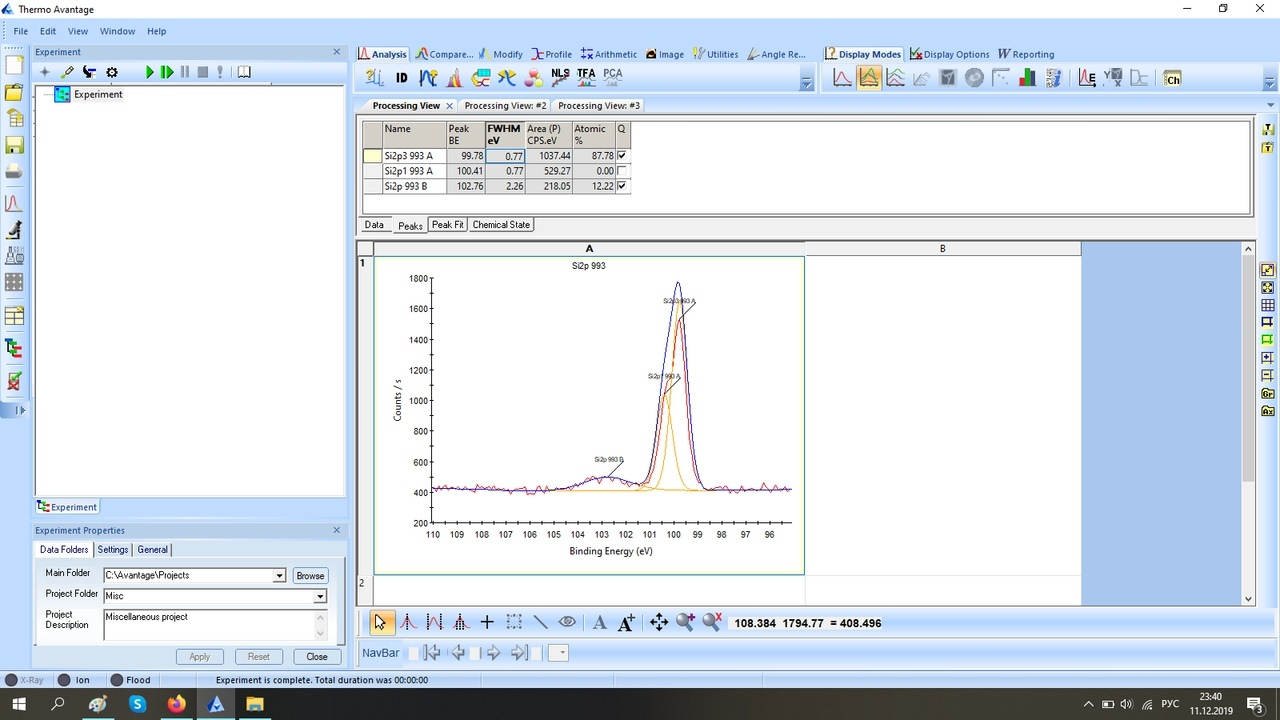
\includegraphics[width=0.6\linewidth]{1.jpg}
  \caption{Спектр к задаче 1. Вид из интерфейса программы. Спектр после роста на подложке слоя $ Hf_{0,5} Zr_{0,5} O_y $ }
  \label{fig1}
\end{figure}


\textbf{Решение:} Воспользуемся формулой для интенсивности РФЭС линий $ Si 2p $  от  $ Si  $ и $ SiO_2  $ , соответственно:\\

\begin{equation}
	I_{Si} = Q \lambda_{Si}C_{Si} exp( - \frac{x__{SiO_2}}{\lambda_{SiO_2}cos\Theta})exp( - \frac{x__{HZO}}{\lambda_{HZO}cos\Theta})
\end{equation}

\begin{equation}
	I_{SiO_2} = Q \lambda_{SiO_2}C_{SiO_2} exp( - \frac{x__{SiO_2}}{\lambda_{SiO_2}cos\Theta})exp( - \frac{x__{HZO}}{\lambda_{HZO}cos\Theta})
\end{equation}

\\
Тогда:

$$ \frac{I_{SiO_2}}{ I_{Si}} = \frac{\lambda_{SiO_2}}{\lambda_{Si}} \frac{C_{SiO_2}}{C_{Si}} \frac{1- exp( - \frac{x__{SiO_2}}{\lambda_{SiO_2}cos\Theta} ) } {exp( - \frac{x__{SiO_2}}{\lambda_{SiO_2}cos\Theta} )} $$


Откуда получается при подстановке:
\begin{equation}
	Y = - \frac{x__{SiO_2}}{\lambda_{SiO_2}cos\Theta} =  - 0.33
\end{equation}

А толщина оксида:

\begin{equation}
	X = 6.031\times 10^{-9} \approx 0.6 nm
\end{equation}



\section{Задача 2}
\textbf{Задание:} Зафитировать спектр $ Si 2p $, полученный после роста на подложке кремния слоя
$ Hf_{0,5} Zr_{0,5} O_y $ и $ Ti $ , определить толщину оксида (слайды 9,10)



\begin{figure}[H]
	\centering
	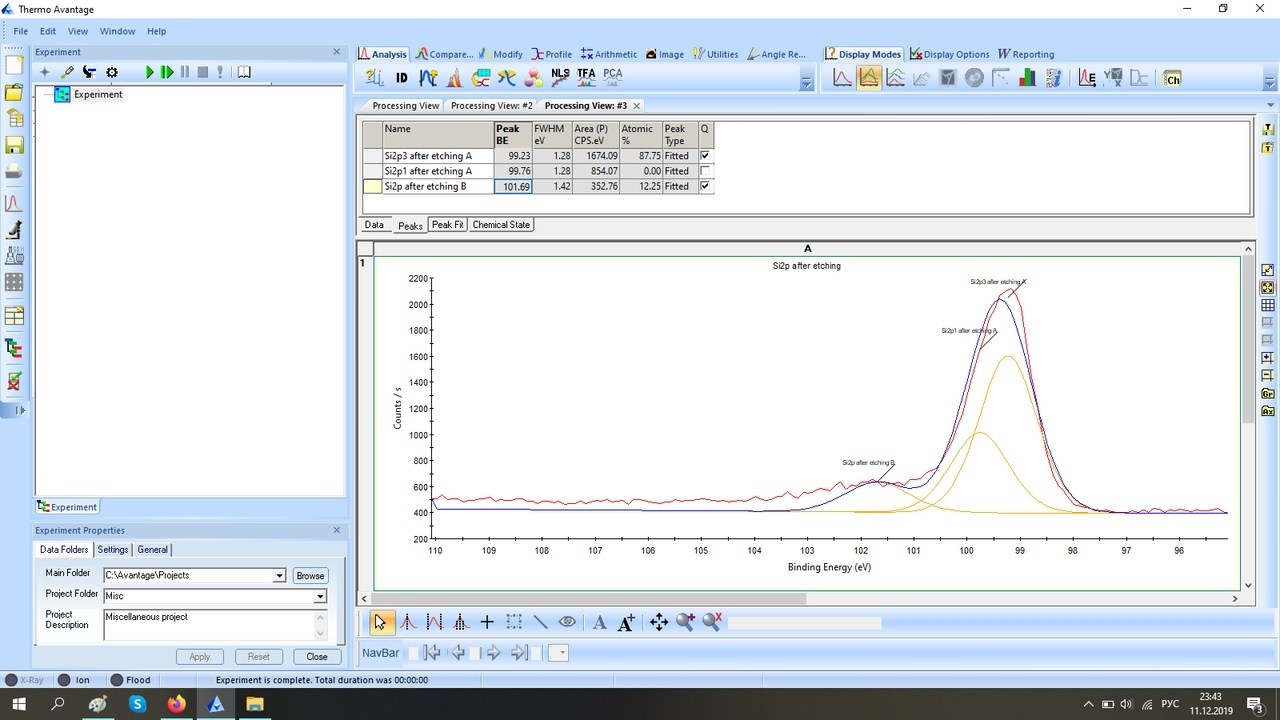
\includegraphics[width=0.8\linewidth]{2.jpg}
	\caption{Спектр к задаче 2. Вид из интерфейса программы.}
	\label{fig2}
\end{figure}

$$ x = - log(\frac{1007647}{725439}) $$


$$  log(\frac{1007647}{725439}) =  \frac{y__{SiO_2}}{\lambda_{SiO_2}cos\Theta} $$

$$ y \approx 6.04721 \times 10^{-11} \approx 0.6 nm $$




\end{document}